\documentclass{article}
\usepackage[margin=1in]{geometry}
\usepackage{fancyhdr}
\usepackage{graphicx}
\usepackage{amsmath}
\usepackage{amssymb}
\usepackage{breqn}
\usepackage{array}
\graphicspath{ {images/} }

\usepackage{tikz}
\newcommand*\circled[1]{\tikz[baseline=(char.base)]{
            \node[shape=circle,draw,inner sep=2pt] (char) {#1};}}

\pagestyle{fancy}
\lhead{BME 384}
\rhead{Pascale Walters 20566177\\
		Dipika Sikka 20564939}

\begin{document}

\begin{center}\underline{\huge Hands-On Fluids Challenge}\end{center}

\textbf{Magnitude of the force that must be applied on the piston}

Mass balance on the control volume (constant flow rate):
\[ v_{1}A_{1} = v_{2}A_{2} \]
\[ v_{1}\pi{R}^2 = v_{2}\pi{R_{o}}^2 \]
\[ \Rightarrow v_{2} = v_{1} \left(\frac{R}{R_{o}}\right)^2 \tag{1} \label{eq:1} \]

Where $v_{1}$ is the velocity at which the piston is pushed and $v_{2}$ is the velocity of the jet of water as it leaves the needle tip. \\

Bernoulli between \circled{1} and \circled{2}:
\[ \frac{P_{1}}{\rho} + \alpha_{1}\frac{{v_{1}}^2}{2}  + gz_{1} = \frac{P_{2}}{\rho} + \alpha_{2}\frac{{v_{2}}^2}{2}  + gz_{2} + h_{f} \tag{2} \label{eq:2} \]

Where,
\[ P_{2} = P_{atm} + P_{capillary}  = P_{atm} + \frac{\gamma}{R_{o}} \]


Using $v_{2}$ from \eqref{eq:1} and assuming laminar flow ($\alpha_{1} = \alpha_{2} = 2$), \eqref{eq:2} becomes:
\[ \frac{P_{1}}{\rho} + {v_{1}}^2 = \frac{P_{atm} + \frac{\gamma}{R_{o}}}{\rho} + {v_{1}}^2\left(\frac{R}{R_{o}}\right)^4  + gl_{needle} + h_{f} \]

Laminar flow can be assumed because the diameter of the needle is very small and the speed of the water is relatively low.

Solving for $P_{1}$,
\[ P_{1} = P_{atm} + \frac{\gamma}{R_{o}} + \rho{v_{1}}^2\left[\left(\frac{R}{R_{o}}\right)^4  - 1 \right] + \rho gl_{needle} + \rho h_{f} \tag{3} \label{eq:3} \]

All values are known in this equation, except for $h_{f}$. The losses due to friction are given as:
\[ h_{f} = 4f_{needle} \frac{l_{needle}}{2R_{o}} \frac{{v_{2}}^2}{2} = 4f_{needle} \frac{l_{needle}}{2R_{o}} \frac{{v_{1}}^2}{2} \left(\frac{R}{R_{o}}\right)^2 \tag{4} \label{eq:4} \]

Minor losses will be neglected because they will be much smaller than the major losses, due to the ratio of the length of the needle to its diameter being very large. Since the flow was assumed to be laminar, the friction factor is:
\[ f = \frac{16}{N_{Re}} \tag{5} \label{eq:5} \]

Where $N_{Re}$ is the Reynolds number given by:
\[ N_{Re} = \frac{\rho v_{2} (2R_{o})}{\mu} = \frac{2 \rho v_{1} R^{2}}{\mu R_{o}} \tag{6} \label{eq:6} \]

Substituting \eqref{eq:6} into \eqref{eq:5}:

\[ f = \frac{8 \mu R_{o}}{\rho v_{1} R^{2}} \tag{7} \label{eq:7} \]

Substituting \eqref{eq:7} into \eqref{eq:4}:

\[ h_{f} = \frac{8 \mu R_{o}}{\rho v_{1} R^{2}} \frac{l_{needle}}{R_{o}} {v_{1}}^2 \left(\frac{R}{R_{o}}\right)^2 \]
\[ h_{f} = \frac{8 \mu l_{needle} v_{1} }{\rho {R_{o}}^2} \tag{8} \label{eq:8} \]

Substituting \eqref{eq:8} into \eqref{eq:3}:
\[ P_{1} = P_{atm} + \frac{\gamma}{R_{o}} + \rho{v_{1}}^2\left[\left(\frac{R}{R_{o}}\right)^4  - 1 \right] + \rho gl_{needle} + \frac{8 \mu l_{needle} v_{1} }{{R_{o}}^2} \tag{9} \label{eq:9} \]

Free body diagram of the forces acting on the piston:

Where $F$ is the applied force to the piston, $F_{s}$ is the sliding friction of the piston on the inside of the syringe and $P_{1}A_{1}$ is the force due to the pressure of the water in the syringe. From Newton's second law,
\[ \Sigma F = ma \]

For the piston to move at a constant velocity,
\[ \Sigma F = 0 \]
\[ \therefore F = F_{s} + P_{1}A_{1} \tag{10} \label{eq:10} \]

Substituting \eqref{eq:9} into \eqref{eq:10},
\[ F(v_{1}) = F_{s} + \left[P_{atm} + \frac{\gamma}{R_{o}} + \rho{v_{1}}^2\left[\left(\frac{R}{R_{o}}\right)^4  - 1 \right] + \rho gl_{needle} + \frac{8 \mu l_{needle} v_{1} }{{R_{o}}^2} \right] \pi R^{2}\]

As determined experimentally, $F_{s} = 35.6 \ N$. Substituting in other known values,
\begin{multline*}
F(v_{1}) = 35.6 \ N + \\ \bigg[ 101.325 \times 10^{3} \ Pa + \frac{72 \times 10^{-3} \ N/m}{0.419 \times 10^{-3} \ m} +\left(1000 \ kg/m^3 \right) {v_{1}}^2 \left[\left(\frac{14.25 \times 10^{-3} \ m}{0.419 \times 10^{-3} \ m}\right)^4  - 1 \right] \\ + \left(1000 \ kg/m^3 \right) \left( 9.81 \ m/s^2 \right) \left( 40 \times 10^{-3} \ m \right) + \\ \frac{8 \left( 10^{-3} \ kg/m \cdot s \right) \left( 40 \times 10^{-3} \ m \right) v_{1}}{\left( 0.419 \times 10^{-3} \ m \right)} \bigg] \pi {\left( 14.25 \times 10^{-3} \ m \right)}^{2}
\end{multline*}

\[ \therefore F(v_{1}) = 100.6 + (487.209 \times 10^{-6}) v_{1} + (853.436 \times 10^{3}) {v_{1}}^2 \ N \]

Where $v_{1}$ is in m/s.
\\

\textbf{Experimental Stuff}

\underline{Measuring properties of the syringe}

Using calipers, the dimensions of the syringe were measured and are reported in Table 1.

\begin{center}\textbf{Table 1:} Syringe and needle dimensions. \end{center}
\begin{center}
\begin{tabular}{| c | c |}
\hline
Syringe inner diameter, $2R$ & 28.5 mm \\ 
\hline
Needle inner diameter, $2R_{o}$ & 0.838 mm \\  
\hline
Needle length & 40 mm \\  
\hline
\end{tabular}
\end{center}

\underline{Measuring height}

Height as a function of the velocity applied to the plunger was measured by observing how high a jet of dyed water reached with a known constant velocity.
The experiment was set up by taping a long sheet of paper to a wall that was marked every 5 cm.
The syringe with attached needle was filled with water that had been dyed green to improve its visibility.
As the plunger was pushed with a constant velocity, the height the water reached was recorded with a camera.
After three trials had been performed, the videos were analyzed to determine the velocity at which the plunger moved and the height that was reached by the water.
These values are recorded in Table 2.

\begin{center}\textbf{Table 2:} Experimental and theoretical water height. \end{center}
\begin{center}
\begin{tabular}{| p{1cm} | p{3.6cm} | p{3.6cm} | p{3.6cm} | p{2cm} |}
\hline
\textbf{Trial} & \textbf{Plunger Velocity (m/s)} & \textbf{Observed Water Height (m)} & \textbf{Theoretical Water Height (m)} & \textbf{\% Error} \\
\hline
1 & $1 \times 10^{-3}$ & 0.20 & 0.0944 & 69.4 \% \\
\hline
2 & $1.5 \times 10^{-3}$ & 0.30 & 0.154 & 29.7 \% \\  
\hline
3 & $0.75 \times 10^{-3}$ & 0.16 & 0.325 & 7.71 \% \\  
\hline
\end{tabular}
\end{center}

\underline{Measuring sliding friction force}

To determine the force required to push the piston with a constant velocity, a knowledge of the sliding friction force between the plunger and the walls of the inside of the syringe is required. 
This was defined as the force required to pull the plunger out of the piston after it has overcome static friction.
Taking this measurement requires the assumption that the sliding friction force is the same as the plunger is pulled out of the syringe and pushed into the syringe.

The sliding friction force was measured by attaching the plunger of the syringe to a hanging scale with the use of a string. 
The body of the syringe was held stationary and the handle of the hanging scale was pulled in an upward direction.
Once the plunger was moving with constant velocity, the mass on the scale was recorded in ounces (mass).
This was performed three times with masses of 132 oz., 131 oz. and 121 oz. recorded.
The average of the three masses was taken and this was converted to kilograms, then to newtons (force) as follows:

\[ m_{average} = \frac{132 \ oz. + 131 \ oz. + 121 \ oz.}{3} = 128 \ oz. = 3.63 \ kg \]
\[ F_{s} = m_{average}g = (3.63 \ kg)(9.81 \ m/s^2) = 35.6 \ N \] 

This force was taken as the sliding friction force. Figure 1 shows the experimental procedure.

\begin{center}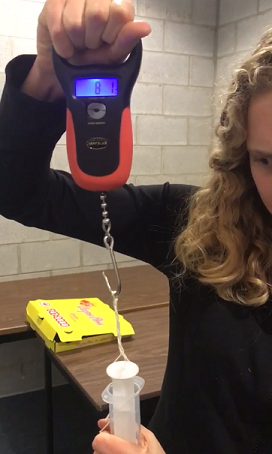
\includegraphics{MeasuringSlidingFriction.png}\end{center}
\begin{center}\textbf{Figure 1:} Measuring sliding friction force. \end{center}

\end{document}